\documentclass[tikz,border=6pt]{standalone}

\usepackage[T1]{fontenc}
\usepackage[utf8]{inputenc}
\usepackage{helvet}
\renewcommand{\familydefault}{\sfdefault}
\usepackage{tikz}
\usetikzlibrary{arrows.meta,positioning,fit,backgrounds,calc}

\definecolor{ctrlblue}{HTML}{4E79A7}
\definecolor{afegreen}{HTML}{59A14F}
\definecolor{timingorange}{HTML}{F28E2B}
\definecolor{triggerred}{HTML}{E15759}
\definecolor{spyteal}{HTML}{76B7B2}
\definecolor{transportpurple}{HTML}{9C755F}
\definecolor{descriptorgold}{HTML}{EDC948}
\definecolor{softgray}{HTML}{F4F4F4}
\definecolor{linegray}{HTML}{5A5A5A}

\tikzset{
  block/.style={
    draw=linegray,
    rounded corners=3pt,
    thick,
    minimum width=3.2cm,
    minimum height=1.15cm,
    align=center,
    font=\sffamily\small,
    fill=white
  },
  subblock/.style={
    draw=linegray,
    rounded corners=2pt,
    semithick,
    minimum width=2.65cm,
    minimum height=0.8cm,
    align=center,
    font=\sffamily\scriptsize,
    fill=white
  },
  flow/.style={-{Latex[length=2.4mm]}, thick, draw=linegray},
  ctrl/.style={-{Latex[length=2.1mm]}, semithick, dashed, draw=ctrlblue},
  note/.style={font=\sffamily\scriptsize, text=linegray, align=center}
}

\begin{document}
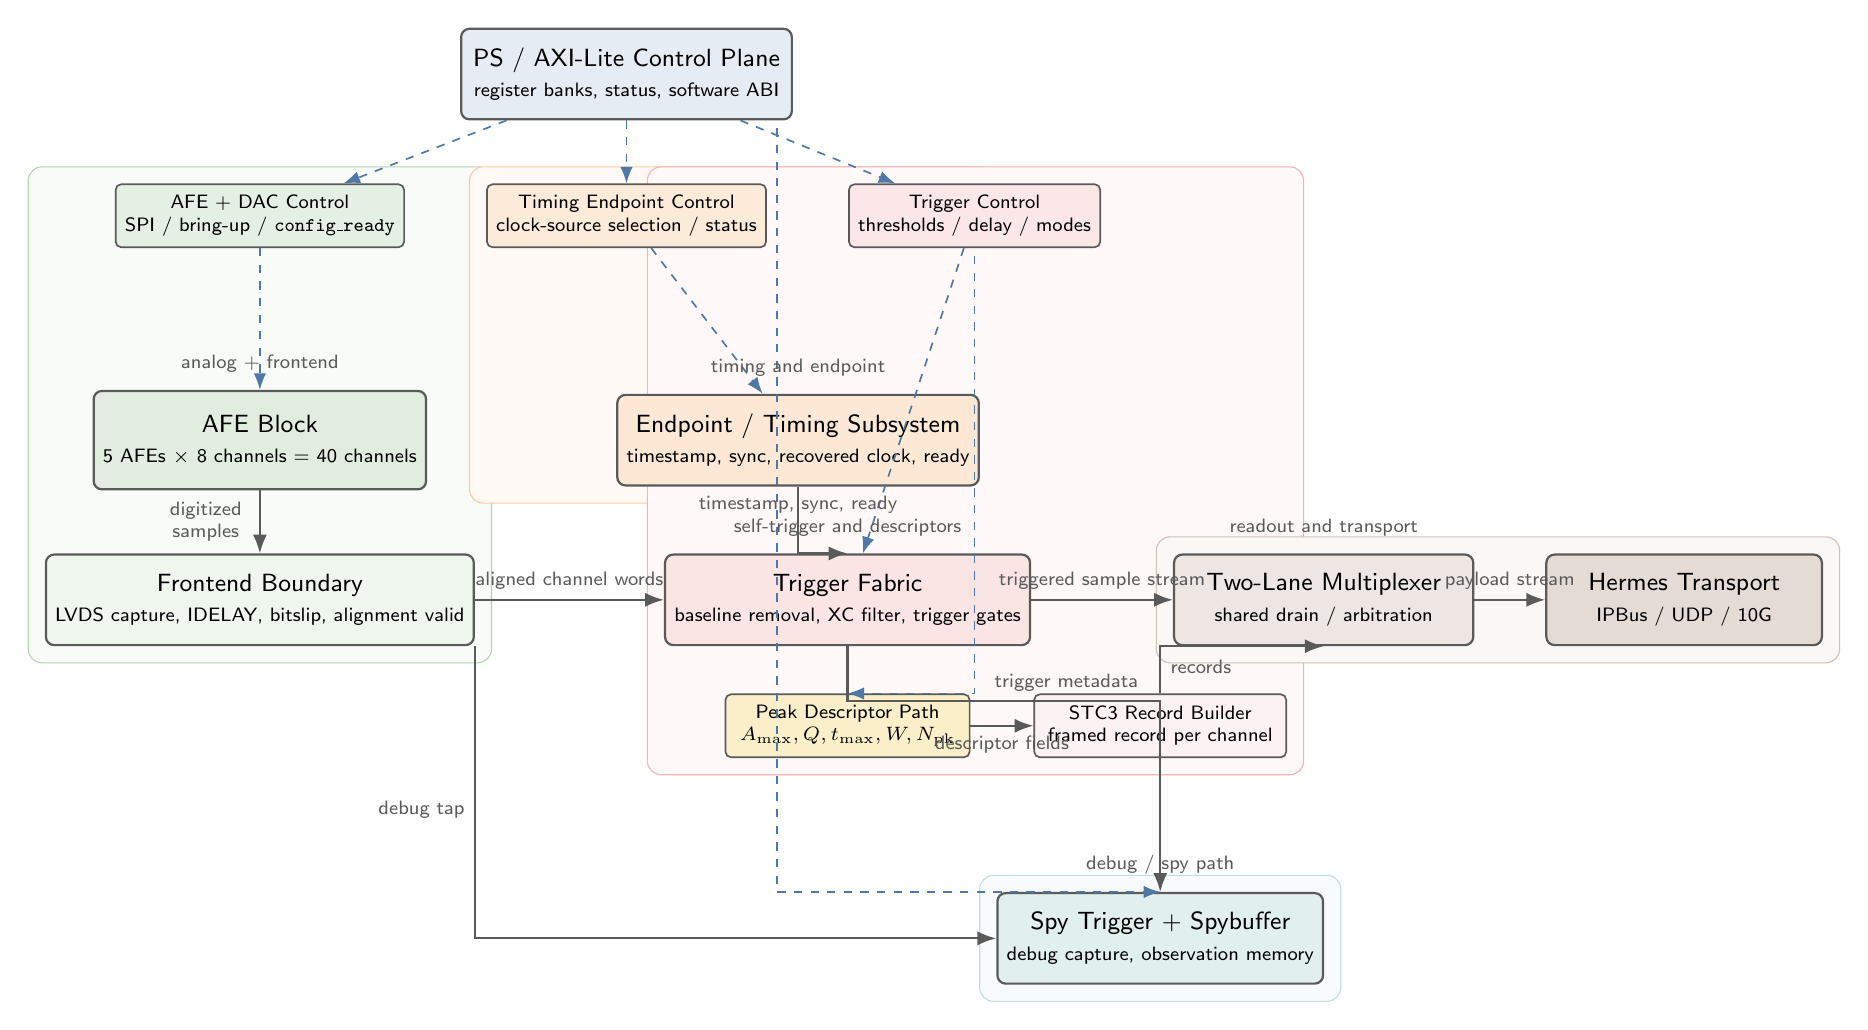
\begin{tikzpicture}[node distance=8mm and 9mm]

% Sources and control
\node[block, fill=ctrlblue!14, minimum width=4.2cm] (ps) {PS / AXI-Lite Control Plane\\\scriptsize register banks, status, software ABI};
\node[subblock, fill=afegreen!16, below left=of ps, xshift=0.2cm] (analog) {AFE + DAC Control\\SPI / bring-up / \texttt{config\_ready}};
\node[subblock, fill=timingorange!18, below=of ps] (endpointctrl) {Timing Endpoint Control\\clock-source selection / status};
\node[subblock, fill=triggerred!14, below right=of ps, xshift=-0.2cm] (triggerctrl) {Trigger Control\\thresholds / delay / modes};

% Left capture chain
\node[block, fill=afegreen!18, below=18mm of analog, minimum width=3.9cm, minimum height=1.25cm] (afe) {AFE Block\\\scriptsize 5 AFEs $\times$ 8 channels = 40 channels};
\node[block, fill=afegreen!10, below=of afe, minimum width=3.9cm] (frontend) {Frontend Boundary\\\scriptsize LVDS capture, IDELAY, bitslip, alignment valid};

% Timing
\node[block, fill=timingorange!20, right=24mm of afe, minimum width=3.9cm] (endpoint) {Endpoint / Timing Subsystem\\\scriptsize timestamp, sync, recovered clock, ready};

% Trigger chain
\node[block, fill=triggerred!16, right=24mm of frontend, minimum width=4.3cm] (trigger) {Trigger Fabric\\\scriptsize baseline removal, XC filter, trigger gates};
\node[subblock, fill=descriptorgold!30, below=6mm of trigger, minimum width=3.1cm] (descriptor) {Peak Descriptor Path\\\scriptsize $A_{\max}, Q, t_{\max}, W, N_{\mathrm{pk}}$};
\node[subblock, fill=triggerred!8, right=8mm of descriptor, minimum width=3.2cm] (builder) {STC3 Record Builder\\\scriptsize framed record per channel};

% Readout / transport
\node[block, fill=transportpurple!18, right=18mm of trigger, minimum width=3.8cm] (mux) {Two-Lane Multiplexer\\\scriptsize shared drain / arbitration};
\node[block, fill=transportpurple!26, right=of mux, minimum width=3.5cm] (hermes) {Hermes Transport\\\scriptsize IPBus / UDP / 10G};

% Spy path
\node[block, fill=spyteal!22, below=17mm of builder, minimum width=3.9cm] (spy) {Spy Trigger + Spybuffer\\\scriptsize debug capture, observation memory};

% Background group regions
\begin{pgfonlayer}{background}
  \node[draw=afegreen!45, rounded corners=5pt, fill=afegreen!4,
        fit=(analog)(afe)(frontend), inner sep=6pt] {};
  \node[draw=timingorange!45, rounded corners=5pt, fill=timingorange!5,
        fit=(endpointctrl)(endpoint), inner sep=6pt] {};
  \node[draw=triggerred!45, rounded corners=5pt, fill=triggerred!4,
        fit=(triggerctrl)(trigger)(descriptor)(builder), inner sep=6pt] {};
  \node[draw=transportpurple!45, rounded corners=5pt, fill=transportpurple!5,
        fit=(mux)(hermes), inner sep=6pt] {};
  \node[draw=spyteal!45, rounded corners=5pt, fill=spyteal!5,
        fit=(spy), inner sep=6pt] {};
\end{pgfonlayer}

% Control arrows
\draw[ctrl] (ps) -- (analog);
\draw[ctrl] (ps) -- (endpointctrl);
\draw[ctrl] (ps) -- (triggerctrl);
\draw[ctrl] (analog) -- (afe);
\draw[ctrl] (endpointctrl) -- (endpoint);
\draw[ctrl] (triggerctrl) -- (trigger);
\draw[ctrl] ($(triggerctrl.south)+(0,-1mm)$) |- (descriptor.north);
\draw[ctrl] ($(ps.south east)+(-2mm,-1mm)$) |- (spy.north);

% Functional flows
\draw[flow] (afe) -- node[note, left, xshift=-1mm] {digitized\\samples} (frontend);
\draw[flow] (frontend) -- node[note, above] {aligned channel words} (trigger);
\draw[flow] (endpoint) |- node[note, pos=0.28, above] {timestamp, sync, ready} (trigger.north);
\draw[flow] (trigger) -- node[note, above] {triggered sample stream} (mux);
\draw[flow] (descriptor) -- node[note, below] {descriptor fields} (builder);
\draw[flow] (builder) |- node[note, pos=0.28, right] {records} (mux.south);
\draw[flow] (mux) -- node[note, above] {payload stream} (hermes);
\draw[flow] (frontend.south east) |- node[note, pos=0.28, left] {debug tap} (spy.west);
\draw[flow] (trigger.south) -- ++(0,-7mm) -| node[note, pos=0.35, above] {trigger metadata} (spy.north);

% Labels
\node[note, above=1mm of afe] {analog + frontend};
\node[note, above=1mm of endpoint] {timing and endpoint};
\node[note, above=1mm of trigger] {self-trigger and descriptors};
\node[note, above=1mm of mux] {readout and transport};
\node[note, above=1mm of spy] {debug / spy path};

\end{tikzpicture}
\end{document}
